
\chapter{序言}
\thispagestyle{empty}

\setlength{\fboxrule}{0pt}\setlength{\fboxsep}{0cm}
\noindent\shadowbox{
\begin{tcolorbox}[arc=0mm,colback=lightblue,colframe=darkblue,title=学习目标与要求]
%kai\textcolor{darkblue}{1.~~对抗学习.} \\ 

\end{tcolorbox}}
\setlength{\fboxrule}{1pt}\setlength{\fboxsep}{4pt}

\section{算法演进之路}

从pc互联网到移动互联网,阿里巴巴电商平台一路高歌猛进,
数据规模,计算能力都发生了天翻地覆的变化;
如图1所示,
\begin{figure}[h]
\centering
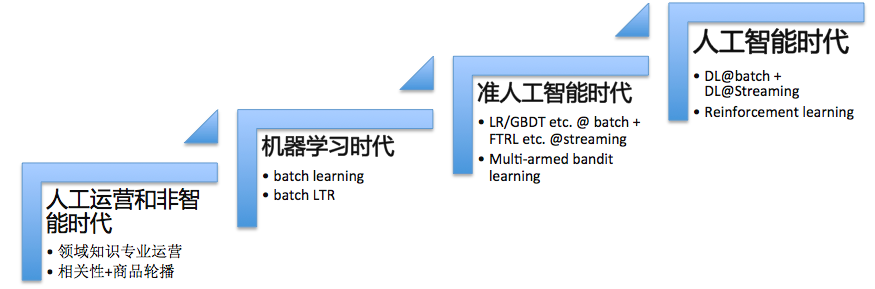
\includegraphics[totalheight=2.0in]{fig/searchAlgoRoadmap.png}
\caption{搜索智能化体系演进图} \label{fig:gansamples}
\end{figure}

\subsection{人工+弱算法时代} 
这个时代的关键词:\textbf{规则 + 轮播}

算法及模型在搜索和推荐系统领域占据统治地位之前,具有领域知识的专业运营和
产品往往充当信息展示规则的制定者,根据主观的判断和对市场的敏锐度来制定
查询词背后的商品展示逻辑。“人工规则”的好处是容易理解和操控,坏处则不言而喻,
随着平台规模的增大,简单规则无法精细的表达人货匹配的效率,并且容易被一些
不良商家利用规则来扰乱市场秩序;实际上,早期的搜索和推荐系统也会运用一些
基本的算法逻辑来保证信息匹配的正确性和人货匹配的公平性,基于传统搜索
引擎技术的相关性模型,保证用户查询词语商品标题的有效匹配;基于商品成交
与否的销售人气指数模型,保证有助于被消费者接受的商品得到更多的展示机会;
另外还有一个就是系统为了保证让更多商家有机会得到展现,设置的按照虚拟下架
周期为参考的轮播因子,即将下架的商品会得到相对较高的展示机会。
$$
	score(item)=1-\frac{ItemOffshelfTime-QueryTime}{secondsOfTwoweek}\times(\frac{docFound}{delta})
$$

这个时代遗留下来几个关键问题需要解决:
\begin{description}
	\item 
\end{description}

\subsection{大规模机器学习时代}
这个时代的关键词:\textbf{big data,offline + shallow model}

随着平台规模的扩大,大规模商家入驻,积极的在平台上打理店铺,发布商品,
相对结构化的商品组织体系,类目结构,属性信息,基于商品为key的销量的累积,
评论的累积,这些为更好的理解商品积累了重要的原始数据资料;
消费者通过搜索产品的各级页面与平台的互动越来越频繁;
数据的组织形成了以人为key的结构体系,反馈信号也得以在闭环系统中有效的流转;
所有的这些都为理解用户积累了重要的数据资料。
有效数据的积累为大规模运用机器学习技术解决问题提供了必要的土壤。

这方面各大互联网公司和科研机构,学校公开发表出来的有参考价值的工作有不少,
典型的有价值工作,logistic regression,gbdt; 




\subsection{准人工智能时代}
这个时代关键词:\textbf{big data,online,deep model }



\subsection{人工智能时代} 
这个时代的关键词: \textbf{big data,online,deep model,decision learning}

淘宝搜索算法技术演进之路可以分为四个阶段,如图所示: 




\section{评估体系} 


\section{技术体系进展} 
recency-sensitive ranking
location-sensitive ranking 





\begin{thebibliography}{99}
\addcontentsline{toc}{chapter}{\protect\numberline{}{\hspace{-1.5em}参考文献}}
\markboth{参考文献}{参考文献}
\bibitem{1} Bilinear+LinUcb的个性化主题推荐, http://www.atatech.org/articles/67847
\bibitem{2} 依托搜索技术的个性化平台之路, http://www.atatech.org/articles/13748
\bibitem{3} 用户意图预估之实时意图篇, http://www.atatech.org/article/detail/12636/152
\bibitem{4} 知人知面需知心——论人工智能技术在推荐系统中的应用,http://geek.csdn.net/news/detail/112318
\bibitem{5} Google, Ad Click PredictionL a View from the trenches. pCTR使用LR,通过
FTRL Proximal 算法实现在线模型更新,频率学派,写的很细致,也有工程细节
\bibitem{6} Bing, Web-Scale Bayesian Click-through Rate Prediction for sponsored 
Search Advertising in Microsoft‘s Bing Search Engine。 Online Bayesian Probit Regression,贝叶斯学派,涉及采样算法的模型
\bibitem{7} Facebook, Practical Lessones from Predicting Clicks on Ads Clicks 
on Ads at facebook。 DT+LR。 和GBDT非常类似,不同之处在于用LR重新训练了每棵树投票的权重,
人气很旺的xgboost,在这一块也是做了优化,利用二阶导数信息得到更快收敛的步长。 缺点是
处理不了高纬度特征,处理连续值特征有优势。
\bibitem{8} 我所经历的大数据平台发展史(三):互联网时代 • 上篇, http://www.infoq.com/cn/articles/the-development-history-of-big-data-platform-paet02, 
\bibitem{9} Fast and Reliable Online Learning to Rank
for Information Retrieval, https://khofm.files.wordpress.com/2013/04/thesis-katja-hofmann-online-learning.pdf
\bibitem{10} Dawei Yin, etc.., Ranking Relevance in Yahoo Search, KDD'16 
\bibitem{11} C.J.C. Burges, FromRankNettoLambdaRanktoLambdaMART: An overview, Technical 
report, Microsoft Research 2010
\bibitem{12} Z. Cao, T. Qin, etc.., Learningtorank: from pairwise approach to listwise approach, ICML'07 
\bibitem{13} A. Dong, Y. Chang, etc.., Towards recency ranking in web search. In WSDM'10. 


\end{thebibliography}

 
